\documentclass[11pt]{article}

\usepackage{graphicx}
\usepackage{amsmath}
\usepackage{amssymb}
\usepackage{siunitx}
\usepackage[a4paper, total={6.3in, 10.5in}]{geometry}
\usepackage{titling}
\usepackage{listings}
\usepackage{float}
\usepackage{subcaption}
\usepackage{pdfpages}
\usepackage{bbm}
\usepackage{amsfonts}

\graphicspath{{figures/}}
\title{\vspace{-2cm}4F13 Coursework 3 - Latent Dirichlet Allocation}
\preauthor{}
\author{}
\postauthor{}
\date{December 2024}

\setlength{\belowcaptionskip}{-5pt}

\begin{document}

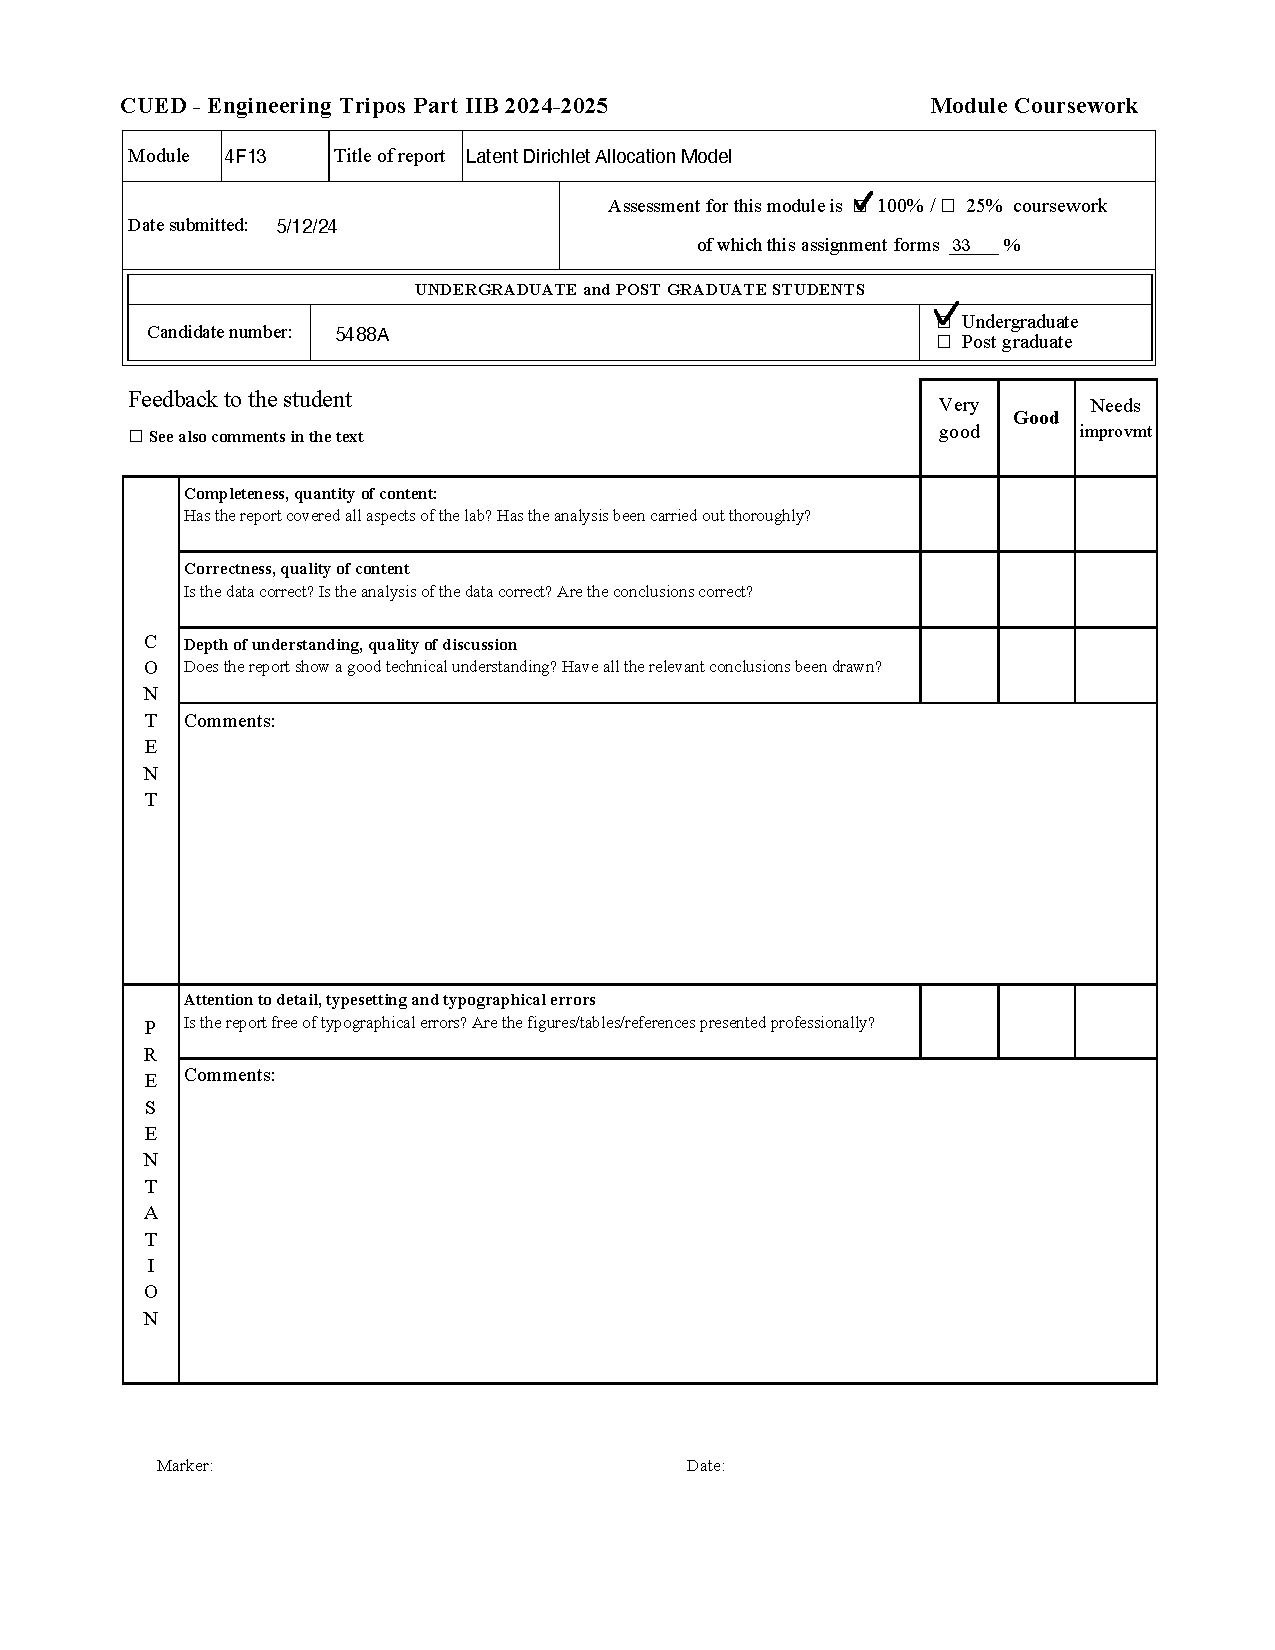
\includepdf[pages={1}]{coversheet}

\setcounter{page}{1}

\maketitle

\section{Task A}

We start by using a simple bag of words model to represent the entire training dataset, $\mathcal{A}$. The likelihood, Equation \ref{eq:A_likelihood}, is a multinomial over the $M$ words in the vocabulary. $k_m$ is the count of word $m$ in the training dataset and $\pi_m$ is its probability. We collect these elements into vectors $\boldsymbol{k}$ and $\boldsymbol{\pi}$ respectively.
\begin{equation}
    \small
    P(\mathcal{A} | \boldsymbol{\pi}) = N! \prod_{m=1}^{M} \frac{\pi_m^{k_m}}{k_m!}
    \label{eq:A_likelihood}
\end{equation}

To compute a maximum likelihood estimate we can maximise the log likelihood, for easier derivative computation, with a Lagrange multiplier to enforce the constraint that the probabilities sum to 1. We find that the maximum likelihood estimate for $\pi_m$, Equation \ref{eq:A_ML_estimate}, is simply the frequency of word $m$ in the training dataset.
\begin{equation}
    \small
    \begin{aligned}
        \mathcal{L} &= \log(P(\mathcal{A} | \boldsymbol{\pi})) + \lambda (\sum_{m=1}^{M} \pi_m - 1) \\
        \left . \frac{\partial \mathcal{L}}{\partial \pi_i} \right \rvert_{\pi_i^{ML}} &= \frac{k_i}{\pi_i^{ML}} + \lambda^{ML} = 0 \quad \therefore \pi_i^{ML} = - \frac{k_i}{\lambda^{ML}}§ \\
        \sum_{m=1}^{M} \pi_m^{ML} &= \sum_{m=1}^{M} -\frac{k_m}{\lambda^{ML}} = 1 \quad \therefore \lambda^{ML} = -\sum_{m=1}^{M} k_m \\
        \therefore \pi_i^{ML} &= \frac{k_i}{\sum_{m=1}^{M} k_m}
    \end{aligned}
    \label{eq:A_ML_estimate}
\end{equation}
\begin{figure}
    \centering
    \begin{minipage}{0.49\textwidth}
        \centering
        \includegraphics[width=\textwidth]{A/most_likely}
        \subcaption{20 most likely words.}
        \label{fig:A_most_likely_words}
    \end{minipage}
    \begin{minipage}{0.49\textwidth}
        \centering
        \includegraphics[width=\textwidth]{A/least_likely}
        \subcaption{20 least likely words}
        \label{fig:A_least_likely_words}
    \end{minipage}
    \caption{Maximum likelihood estimates of multinomial probabilities from dataset $\mathcal{A}$.}
    \label{fig:A_ML_estimates}
\end{figure}

We see in Figure \ref{fig:A_ML_estimates} that the most likely word is `bush' with a probability of $0.0141$ and there are multiple words in the vocabulary that do not appear in the training dataset and therefore have a probability of $0$. 

Consider a test dataset, $\mathcal{B}$, with length $N_{\mathcal{B}}$. The test set of maximum likelihood would be simply be $N_{\mathcal{B}}$ copies of the most likely word in $\boldsymbol{\pi}^{ML}$, ``bush'' in our case when trained on $\mathcal{A}$. The log likelihood of this test set would be $N_{\mathcal{B}} \log(\pi_{\text{bush}}^{ML}) = -4.26 N_{\mathcal{B}}$.

Furthermore we notice that the minimum likelihood test set would be any test set that contains words not in the training dataset. This is because the probability of any word not in the training dataset is $0$ and therefore the log likelihood of any test set containing such a word would be $-\infty$. This is a limitation of the ML estimate model as no valid test set should have probability $0$.
\section{Task B}
To combat this issue we can perform Bayesian inference. We assume a symmetric Dirichlet prior for our probability vector $\boldsymbol{\pi}$, Equation \ref{eq:B_prior}, with concentration parameter $a$.
\begin{equation}
    \small
    \begin{aligned}
        p(\boldsymbol{\pi}) = \text{Dir}(\boldsymbol{\pi} | \boldsymbol{\alpha} = \boldsymbol{1} a) = \frac{1}{\text{B}(\boldsymbol{1} a)} \prod_{m=1}^{M} \pi_m^{a - 1}
    \end{aligned}
    \label{eq:B_prior}
\end{equation}
Using the same likelihood, Equation \ref{eq:A_likelihood}, we find that the posterior distribution of $\boldsymbol{\pi}$ is also a Dirichlet distribution, Equation \ref{eq:B_posterior}, with parameter $\boldsymbol{\alpha} = \boldsymbol{k} + \boldsymbol{1} a$.
\begin{equation}
    \small
    \begin{aligned}
        p(\boldsymbol{\pi} | \mathcal{A}) &\propto p(\mathcal{A} | \boldsymbol{\pi}) p(\boldsymbol{\pi}) \propto \prod_{m=1}^{M} \pi_m^{k_m + a - 1} \\
        \therefore p(\boldsymbol{\pi} | \mathcal{A}) &= \text{Dir}(\boldsymbol{\pi} | \boldsymbol{\alpha} = \boldsymbol{k} + \boldsymbol{1} a)
    \end{aligned}
    \label{eq:B_posterior}
\end{equation}
We compute the predictive word probability, Equation \ref{eq:B_predictive}, and notice that it is similar to the maximum likelihood estimate but with an initial pseudo count of $a$ for each word. This means that the probability of a words not seen in the training dataset now have non-zero probability, fixing the flaw of the maximum likelihood estimate.
\begin{equation}
    \small
    \begin{aligned}
        p(w = i | \mathcal{A}) &= \int_{|\boldsymbol{\pi}|_1=1} p(w = i | \boldsymbol{\pi}) p(\boldsymbol{\pi} | \mathcal{A}) d\boldsymbol{\pi} \\
          &= \int_{0}^{1} \pi_i p(\pi_i | \mathcal{A}) d\pi_i \\
          &= \mathbbm{E}_{\pi_i|\mathcal{A}}[\pi_i] \\
          &= \frac{a + k_i}{M a + \sum_{m=1}^{M} k_m} = \hat \pi_i \\
    \end{aligned}
    \label{eq:B_predictive}
\end{equation}
For small values of $a$, predictive probabilities with the Bayesian estimate approach those of the maximum likelihood estimate. As $a$ increases, words with probability greater than $\frac{1}{M}$ will decrease in probability and words with probability less than $\frac{1}{M}$ will increase in probability. This is because for large values of $a$ our observations become insignificant compared to the prior so the posterior distribution will approach the prior distribution giving a uniform predictive distribution.

We have added a hyper-parameter $a$ to our model which we wish to choose in an analytical way. We can do this by maximising the marginal likelihood of the training dataset, $\mathcal{A}$, Equation \ref{eq:B_marginal_likelihood}. We plot the log marginal likelihood for different values of $a$ in Figure \ref{fig:C_hyper_parameter_opt} and find that the maximum marginal likelihood occurs at $a = 0.753$. We will use this value in the following task.
\begin{equation}
    \small
    \begin{aligned}
        p(\mathcal{A}) &= \frac{p(\mathcal{A} | \boldsymbol{\pi}) p(\boldsymbol{\pi})}{p(\boldsymbol{\pi} | \mathcal{A})} \\
          &= \frac{\text{B}(\boldsymbol{k} + \boldsymbol{1} a)}{\text{B}(\boldsymbol{1} a)} \\ 
    \end{aligned}
    \label{eq:B_marginal_likelihood}
\end{equation}

\begin{figure}
    \centering
    \includegraphics[width=0.5\textwidth]{C/hyper_parameter_opt}
    \caption{Optimisation of hyper-parameter $a$ using marginal likelihood.}
    \label{fig:C_hyper_parameter_opt}
\end{figure}

\section{Task C}
We wish to compute the probability of a test document, $\mathcal{T}$. We use a categorical distribution, over a multinomial, as a document is not uniquely defined by its word counts, the word order matters too.
\begin{equation}
    \small
    \begin{aligned}
        p(\mathcal{T} | \mathcal{A}) &= \prod_{n=1}^{N_{\mathcal{T}}} p(w_n | \mathcal{A}) \\
          &= \prod_{m=1}^{M} \hat \pi_{w_n}^{k_{w_n}} \\
        \log(p(\mathcal{T} | \mathcal{A})) &=  \boldsymbol{k} \cdot \log(\boldsymbol{\hat \pi})
    \end{aligned}
\end{equation}
For document $2001$ in the test dataset, $\mathcal{B}_{2001}$, we calculate a log probability of $-3689.3$. We are also interested in the per word perplexity of a given document, Equation \ref{eq:C_perplexity}. 
\begin{equation}
    \small
    \begin{aligned}
        \text{Perplexity}(\mathcal{T}) &= \exp(-\frac{\log(p(\mathcal{T} | \mathcal{A}))}{N_{\mathcal{T}}} ) \\
    \end{aligned}
    \label{eq:C_perplexity}
\end{equation}

The per word perplexity of $\mathcal{B}_{2001}$ and the entire test set, $\mathcal{B}$, are given in Table \ref{tab:C_perplexity}. We notice that the per word perplexity of $\mathcal{B}_{2001}$ is greater than that of the whole test set. This indicates that $\mathcal{B}_{2001}$ contains a higher frequency of words that are rare in $\mathcal{A}$ than the rest of the $\mathcal{B}$. The perplexity of a uniform multinomial is simply the size of the vocabulary, $M$, and for long documents this is an upper bound.

\begin{table}
    \centering
    \begin{tabular}{|c|ccc|}
        \hline
         & Document 2001 - $\mathcal{B}_{2001}$ & Test Set - $\mathcal{B}$ & Uniform Multinomial \\
        \hline
        per-word perplexity & $4379.6$ & $2686.1$ & $6906 = M$ \\
        \hline
    \end{tabular}
    \caption{Perplexities of documents.}
    \label{tab:C_perplexity}
\end{table}

\section{Task D}
This model still has a limitation in that it assumes all documents are drawn from the same distribution. However, in the real world documents can be about different topics and therefore have different word distributions. We can use a Mixture of Multinomials model where each document has a latent variable, $z_d$, that determines which of the $K$ topic distributions $\boldsymbol{\beta}_k$ it is drawn from. The latent topic variables are drawn from a categorical distribution with parameter $\boldsymbol{\theta}$. The prior for $\boldsymbol{\theta}$ and each $\boldsymbol{\beta}_k$ are symmetric Dirichlet with parameters $\alpha$ and $\gamma$ respectively. A graphical representation of the model is given in Figure \ref{fig:D_graphical_model}.

\begin{figure}
    \centering
    \includegraphics[width=0.8\textwidth]{D/graphical_model}
    \caption{Mixture of Multinomials model.}
    \label{fig:D_graphical_model}
\end{figure}
We perform Gibbs sampling of the latent variable using the training documents, $\mathcal{A}$. We set our prior hyper-parameters to $\alpha = 1$ and $\gamma = 0.1$ and run the Gibbs sampler for $50$ iterations with $K=20$. We compute topic posterior, $\boldsymbol{\hat \theta}^{(i)}$, at each Gibbs iteration $i$ using Equation \ref{eq:D_topic_posterior}, where $D_{\mathcal{A}}$ is the number of documents in $\mathcal{A}$. Similar to the previous multinomial posteriors, it is simply the frequency of each topic across the documents adjusted with a pseudo count of the prior, $\alpha$.

\begin{equation}
    \small
    \begin{aligned}
        (\boldsymbol{\hat \theta}^{(i)})_k = \frac{\alpha + \sum_{d=1}^{D_{\mathcal{A}}} \mathbbm{1}(z_{d} = k)}{K \alpha + D_{\mathcal{A}}}
    \end{aligned}
    \label{eq:D_topic_posterior}
\end{equation}
We plot the evolution of the topic posterior for 3 different seeds in Figure \ref{fig:D_topic_proportions}. We notice a burn in period of about $20$ iterations before the sampler reaches the high probability region of our posterior. We expect the the same that the same ``concepts'' will not be assigned to the same topic variable across different seeds as the topic variables are arbitrary. 
However, we also see that the final topic proportions are different across seeds. This indicates that that the topic posterior distribution is multimodal and the Gibbs sampler is not doing a good job of fully exploring the posterior distribution. In fact, in Figure \ref{fig:D_topic_1} we see the Gibbs sampler switching to a different mode after iteration $40$. The mode of the posterior distribution that ends up being converging to is dependant on the seed. We could consider alternative MCMC methods to more fully explore the posterior distribution. However, we notice that for all seeds the test set perplexity is similar, indicating that the different modes are equally good fits.
\begin{figure}
    \centering
    \begin{minipage}{0.32\textwidth}
        \centering
        \includegraphics[width=\textwidth]{D/mixing_proportions_seed_0}
        \subcaption{Seed = 0, Perplxty = $2117.9$}
        \label{fig:D_topic_0}
    \end{minipage} 
    \begin{minipage}{0.32\textwidth}
        \centering
        \includegraphics[width=\textwidth]{D/mixing_proportions_seed_10}
        \subcaption{\small{Seed = 10, Perplxty = $2112.6$}}
        \label{fig:D_topic_1}
    \end{minipage}
    \begin{minipage}{0.32\textwidth}
        \centering
        \includegraphics[width=\textwidth]{D/mixing_proportions_seed_100}
        \subcaption{Seed = 100, Perplxty = $2101.2$}
        \label{fig:D_topic_2}
    \end{minipage}
    \caption{Topic proportions at each Gibbs for different seeds, coloured by final proportion. Test set perplexity is given in the caption.}
    \label{fig:D_topic_proportions}
\end{figure}

\section{Task E}
Sometimes a single document can contain more than one topic, therefore, we make a final modification to our model. We allow the topic proportions, $\boldsymbol{\theta}_d$, to vary for each document. The $n$th word in document $d$ is then given a latent topic variable, $z_{nd}$, sampled from $\boldsymbol{\theta}_d$. We still use a symmetric Dirichlet prior with parameter $\alpha$ for each $\boldsymbol{\theta}_d$. This allows each document to be described by and arbitrary mixture of topics and is called Latent Dirichlet Allocation (LDA). The graphical model is given in Figure \ref{fig:E_graphical_model}.

\begin{figure}
    \centering
    \includegraphics[width=0.6\textwidth]{E/graphical_model}
    \caption{Latent Dirichlet Allocation Model.}
    \label{fig:E_graphical_model}
\end{figure}

Again we perform Gibbs sampling, using the same hyper-parameter values as before. We compute the topic posteriors from the Gibbs samples, $\boldsymbol{\hat \theta}_d$, as previously, except now for each document individually. These are plotted for a selection of documents against Gibbs iteration in Figure \ref{fig:E_topic_proportions}.
\begin{equation}
    \small
    \begin{aligned}
        (\boldsymbol{\hat \theta}_d^{(i)})_k = \frac{\alpha + \sum_{n=1}^{N_d} \mathbbm{1}(z_{nd} = k)}{K \alpha + N_d}
    \end{aligned}
\end{equation}

For the documents in Figure \ref{fig:E_topic_proportions} we see that the burn in period is about $20$ iterations. We also notice that there is significant variation in how specific the topic distribution of each document is. Document 21 has a high proportion of a single topic whereas document 1 is more general. The samples of some of the topic probabilities have significant variance and therefore we should average over more iterations to obtain an accurate estimate of the topic proportions.

\begin{figure}
    \centering
    \begin{minipage}{0.32\textwidth}
        \centering
        \includegraphics[width=\textwidth]{E/mixing_proportions_doc_1}
        \subcaption{Document 1}
        \label{fig:E_topics_0}
    \end{minipage}
    \begin{minipage}{0.32\textwidth}
        \centering
        \includegraphics[width=\textwidth]{E/mixing_proportions_doc_11}
        \subcaption{Document 11}
        \label{fig:E_topics_1}
    \end{minipage}
    \begin{minipage}{0.32\textwidth}
        \centering
        \includegraphics[width=\textwidth]{E/mixing_proportions_doc_21}
        \subcaption{Document 21}
        \label{fig:E_topics_2}
    \end{minipage}
    \caption{Posterior topic proportions at each Gibbs iteration for different documents.}
    \label{fig:E_topic_proportions}
\end{figure}

The perplexity of the test set $\mathcal{B}$ computed using the four models we have discussed is given in Table \ref{tab:E_perplexity}. As our models get more complex the perplexity decreases, this indicates that the test set has a higher likelihood under the more complex models. This is good evidence that the more complex models are both giving a better fit and not overfitting as the perplexity is being measured on the unseen test documents.

\begin{table}
    \centering
    \small
    \begin{tabular}{|c|cccc|}
        \hline
         & Maximum Likelihood & Bayes Posterior & Mixture of Multinomials & LDA \\
        \hline
        Perplexity & $\infty$ & $2686.1$ & $2112.6$ & $1681.1$\\
        \hline
    \end{tabular}
    \caption{Entropy of word distributions at each Gibbs iteration.}
    \label{tab:E_perplexity}
\end{table}

To assess convergence of the word posteriors for each topic we can compute the entropy for each topic with our Gibbs samples. We compute the word posterior, $\boldsymbol{\hat \beta}_k^{(i)}$, at each Gibbs iteration $i$ using Equation \ref{eq:E_word_posterior}. $k_{mk}$ is the number of words $m$ assigned to topic $k$ in $\mathcal{A}$. Equation \ref{eq:E_entropy} gives the entropy of the word distribution for each topic. We are using natural logarithms and therefore the units of this entropy are nats.

\begin{equation}
    \small
    \begin{aligned}
        (\boldsymbol{\hat \beta}_k^{(i)})_m = \frac{\alpha + k_{mk}}{M \gamma + \sum_{i=1}^{M} k_{ik}}
    \end{aligned}
    \label{eq:E_word_posterior}
\end{equation}

\begin{equation}
    \small
    \begin{aligned}
        \text{H}(W_k) &= -\sum_{m=1}^{M} p(w = m | \boldsymbol{\hat \beta}_k) \log(p(w = m | \boldsymbol{\hat \beta}_k)) : W_k \sim \text{Cat}(\boldsymbol{\hat \beta}_k) \\
          &= - \boldsymbol{\hat \beta}_k \cdot \log(\boldsymbol{\hat \beta}_k)
    \end{aligned}
    \label{eq:E_entropy}
\end{equation}

We plot the word entropy against Gibbs iteration in Figure \ref{fig:E_entropy}. A uniform distribution has the highest possible entropy and distributions with most probability mass concentrated in a smaller number of words have lower entropy. Therefore entropy of each topic generally decreases with iteration as the word distributions begin uniform and become increasingly specific as they converge to the posterior. The log perplexity $=7.43$ of the test documents is higher than the entropy of any topic. This is expected as the test set is a blend of all topics and thus has higher entropy than any individual topic.

\begin{figure}
    \centering
    \includegraphics[width=0.5\textwidth]{E/entropy}
    \caption{Entropy of word distributions at each Gibbs iteration.}
    \label{fig:E_entropy}
\end{figure}

From Figures \ref{fig:E_topic_proportions} and \ref{fig:E_entropy} we see that about $30$ iterations are adequate to reach convergence for in the posteriors we have computed and therefore running $50$ iterations is reasonable. In Figure \ref{fig:E_entropy} we see that there are about $5$ topics with much lower entropy than the rest. This is evidence that our chosen number of topics, $K = 20$, is sufficient to capture the main distinct topics in the dataset.
\end{document}